\chapter{Latin bitrades}
\label{chap:bitrades}

An $n \times n$ table such that every row and column contains every number in $[n]$ exactly once is a well-known combinatorial object called \emph{latin square}. In this chapter we define \emph{latin bitrade}, which can be thought of as an object of differences between two latin squares.

To describe a table of elements formally, we use ordered triples $(r,c,s)$ to represent the fact that the cell in row $r$ and column $c$ contains the symbol $s$. For that we use the following notation. Let
\begin{itemize}
	\item $R = \{r_1,\dots,r_{|R|}\}$ denote the set of rows,
	\item $C = \{c_1,\dots,c_{|C|}\}$ denote the set of columns, and
	\item $S = \{s_1,\dots,s_{|S|}\}$ denote the set of symbols.
\end{itemize}
We consider only the case when $R$, $C$, and $S$ are finite. As an example, a latin square is formally a subset of $R \times C \times S$ with $R = C = S = [n]$. We shall see this in more detail in a moment.

In this chapter we define only necessary notions for our purposes. For a more comprehensive introduction to latin bitrades we refer the reader to a survey by Cavenagh \cite{Cavenagh08}.

%%%
%%%
%%%
\section{Partial latin squares}

\begin{defn}
\emph{A partial latin square $L$} is a subset of ordered triples from $R \times C \times S$, such that if $(r,c,s),(r',c',s')\in L$ agree on two coordinates, then $(r,c,s) = (r',c',s')$. We say that $L$ is \emph{on} $R \times C \times S$, or that $R \times C \times S$ is \emph{the support} of $L$.
\end{defn}

A partial latin square is usually interpreted as a partially filled $|R| \times |C|$ table. The condition implies that the table is well defined (there is at most one symbol in every cell), and that no symbol repeats itself within a column or a row.

\begin{defn}
\emph{A latin square $L$} is a partial latin square such that $R=C=S$ and every cell in the table is filled. Equivalently, for every $a, a' \in R$ there are unique $r,c,s \in R$ such that
\begin{cosyeqnarray}
	(r, a, a'), (a, c, a'), (a, a', s) \in L.
\end{cosyeqnarray}
\end{defn}

There are two important maps from partial latin squares to partial latin squares: \emph{isotopy} and \emph{conjugacy}.

\begin{defn}
\label{defn:homotopy}
Let $A \subset R_A \times C_A \times S_A$ and $B \subset R_B \times C_B \times S_B$ be partial latin squares. \emph{A homotopy} $h$ is defined by a triple of maps
\cosyalig{
	h_R : R_A \rightarrow R_B, \quad
	h_C : C_A \rightarrow C_B,\quad
	h_S : S_A \rightarrow S_B
}%
such that 
$$\begin{array}{ c c c c }
h: &	A & \rightarrow & B \\
	&	(r,c,s) & \mapsto & \big(h_R(r), h_C(c), h_S(s)\big).
\end{array}$$
We write $h = (h_R, h_C, h_S)$. A homotopy is \emph{trivial} if there is only one point in its image. \emph{An isotopy} is a homotopy with homotopic inverse.
\end{defn}

\begin{exmp}
Partial latin squares on Figure \ref{fig:isotopic-pls} are isotopic. The set of rows, columns and symbols is the same for both. The isotopy is given by
\begin{cosyitemize}
	\item $h_R$ is identity,
	\item $h_C$ rotates middle three columns,
	\item $h_S(1) = 2,\ h_S(2) = 4,\ h_S(3) = 1,\ h_S(4) = 3,\ h_S(5) = 5$.
\end{cosyitemize}%

\begin{figure}[htb]
	\centering
	\begin{minipage}{.30\linewidth}
		\begin{center}
		\begin{tabular}{| c c c c c |}
			\hline
1 & 3 &   & 2 &   \\
4 &   &   & 1 & 3 \\
  & 4 &   & 5 &   \\
  & 5 & 1 &   & 4 \\
			\hline
		\end{tabular} \\
		\bigskip
		$A$
		\end{center}
	\end{minipage}
	\begin{minipage}{.30\linewidth}
		\begin{center}
		\begin{tabular}{| c c c c c |}
			\hline
2 &   & 4 & 1 &   \\
3 &   & 2 &   & 1 \\
  &   & 5 & 3 &   \\
  & 2 &   & 5 & 3 \\
			\hline
		\end{tabular} \\
		\bigskip
		$B$
		\end{center}
	\end{minipage}
	\caption{Isotopic partial latin squares.}
	\label{fig:isotopic-pls}
\end{figure}

\end{exmp}%

\begin{defn}
Let $A \subset R \times C \times S$ be a partial latin square and $\sigma$ be a permutation of the 3-element set $\{R,C,S\}$. Then the partial latin square
\begin{cosyeqnarray}
	\{(a_{\sigma(R)}, a_{\sigma(C)}, a_{\sigma(S)}) \mid (a_R, a_C, a_S) \in A)\}
\end{cosyeqnarray}
is said to be \emph{conjugated} with $A$.
\end{defn}

Note that there are six conjugacies, each one corresponding to a permutation of $\{R,C,S\}$.

\begin{defn}
Two partial latin squares are from the same \emph{main class} if one can be obtained from the other by composition of conjugacy and isotopy.
\end{defn}


%%%
%%%
%%%
\section{Latin bitrades}
\label{sec:latin-bitrades}

Now we can define a latin bitrade.

\begin{defn}
\emph{A latin bitrade} is a pair $(T, T')$ of partial latin squares on $R \times C \times S$ which are disjoint and for every $(r,c,s) \in T$ (respectively, $T'$) there exist unique $r', c', s'$ such that
\begin{cosyeqnarray}
	(r',c,s), (r,c',s), (r,c,s') \in T' \textrm{ (respectively, $T$)}.
\end{cosyeqnarray}%
Let us call $T$ and $T'$ \emph{latin trades}. Elements of $T$ and $T'$ can be paired with respect to the first two coordinates. Therefore $|T| = |T'|$ and we shall call this number the \emph{size} of the bitrade (or a trade).
\end{defn}

From the tabular point of view, a latin bitrade is a pair of partial latin squares such that they occupy the same cells, but the symbols in corresponding rows and columns are permuted. Moreover, no symbol is at the same position in both of the tables.

\begin{exmp}
The two partial latin squares $(T, T')$ on Figure \ref{fig:latin-bitrade} form a latin bitrade. The example is adapted from \cite{Cavenagh08}.

\begin{figure}[htb]
	\centering
	\begin{minipage}{.30\linewidth}
		\begin{center}
		\begin{tabular}{| c c c c |}
			\hline
  & 1 & 2 & 3 \\
1 & 0 & 3 &   \\
2 &   & 0 & 1 \\
3 & 2 &   & 0 \\
			\hline
		\end{tabular} \\
		\bigskip
		$T$
		\end{center}
	\end{minipage}
	\begin{minipage}{.30\linewidth}
		\begin{center}
		\begin{tabular}{| c c c c |}
			\hline
  & 2 & 3 & 1 \\
3 & 1 & 0 &   \\
1 &   & 2 & 0 \\
2 & 0 &   & 3 \\
			\hline
		\end{tabular} \\
		\bigskip
		$T'$
		\end{center}
	\end{minipage}
	\caption{A latin bitrade on $\Z_4 \times \Z_4 \times \Z_4$ of size 12.}
	\label{fig:latin-bitrade}
\end{figure}

\end{exmp}%

Note that two latin squares $L$, $L'$ defined on the same set specify a latin bitrade $(L \setminus L', L' \setminus L)$. The partial latin squares in this bitrade are ``differences'' of the two latin squares -- $L\setminus L'$ are cells of $L$ which are different from $L'$, and vice versa.

\begin{defn}
A latin bitrade $(T, T')$ is associated with a graph $G = (V, E)$ such that
\cosyalign{
	V &= T \cup T' \nonumber\\
	E &= \{(t,t') \mid t \in T, t' \in T': \textrm{  $t$ and $t'$ differ at exactly one coordinate}\}.\nonumber
}
We call it the \emph{graph of latin bitrade $(T, T')$}.
\end{defn}

Clearly, the graph is bipartite with partitions $T$ and $T'$. It is also 3-regular from the definition of latin bitrade. Moreover, it is edge 3-colorable, since the edges can be colored depending on the coordinate that $t$ and $t'$ differ at.

With the graph representation it is easier to understand the purpose of definitions in the rest of this section.

\begin{defn}
A latin bitrade is \emph{connected} if its graph is connected. It is \emph{spherical} or \emph{planar}, if its graph is planar.
\end{defn}

\begin{exmp}
\label{exmp:graph-bitrade}
Figure \ref{fig:graph-bitrade} shows a graph of a connected spherical latin bitrade $(T,T')$ of size 6. To distinguish the elements of $T$ and $T'$, the latter are typed in brackets. Solid, dashed and dotted edges join elements which differ at $R$-, $C$- and $S$-coordinate respectively.

\begin{figure}[htb]
\centering
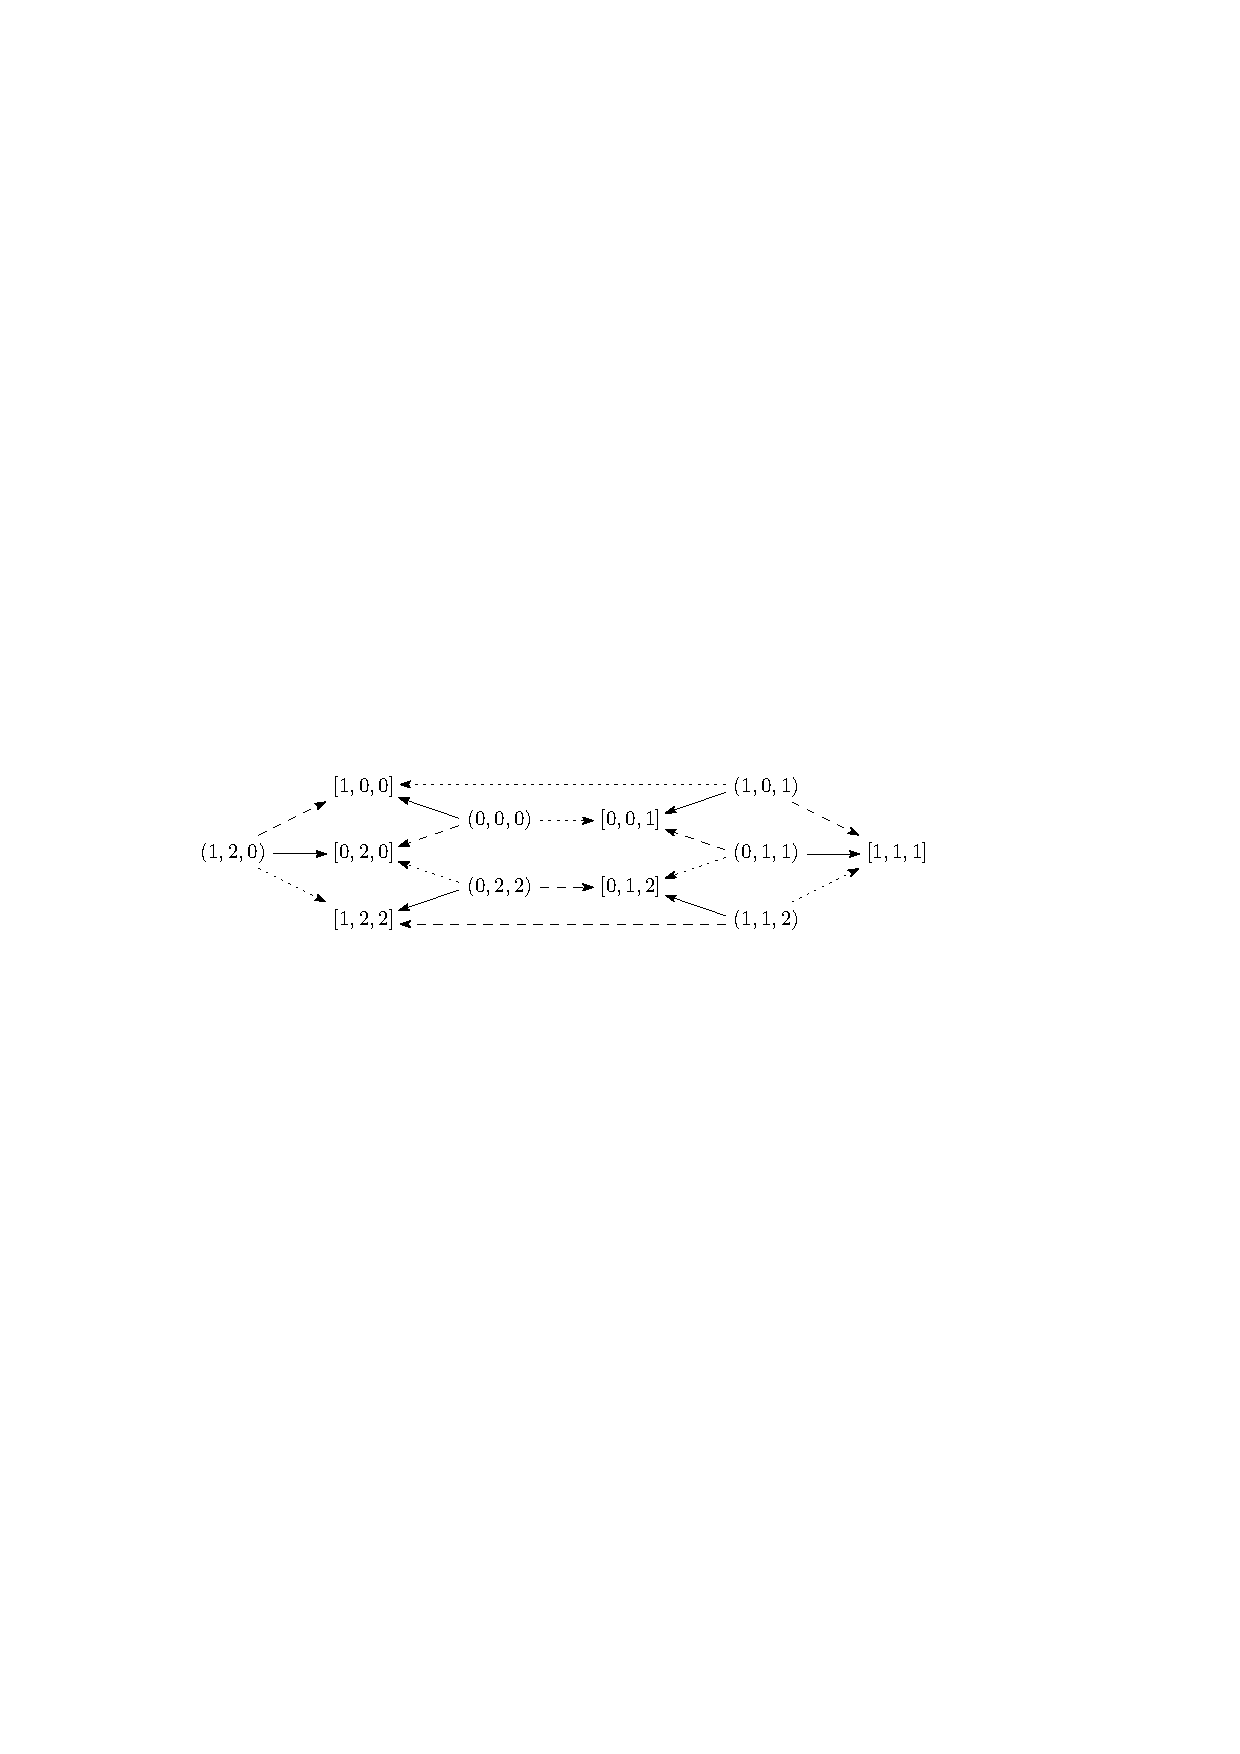
\includegraphics[width=0.9\textwidth]{img/graph_example.pdf}
\caption{Graph of a latin bitrade of size 6 on $\Z_2 \times \Z_3 \times \Z_3$.}
\label{fig:graph-bitrade}
\end{figure}
\end{exmp}%

\noindent
For later use, let us define maps $\sigma_R, \sigma_C, \sigma_S : T \cup T' \rightarrow T \cup T'$ by
\cosyalign{
 	\sigma_R(r,c,s) = (r',c,s) \mbox{ with } r \ne r',\\
 	\sigma_C(r,c,s) = (r,c',s) \mbox{ with } c \ne c', \\
 	\sigma_S(r,c,s) = (r,c,s') \mbox{ with } s \ne s'.
}%
The definition of the latin bitrade implies that these maps are involutions. They correspond to the edges of the graph -- on Figure \ref{fig:graph-bitrade},  $\sigma_R, \sigma_C, \sigma_S$ are represented by solid, dashed and dotted edges respectively.

\begin{lem}
\label{lem:connected-sigma}
A latin bitrade $(T,T')$ is connected if and only if for any $t_1,t_2 \in T \cup T'$ it is possible to get $t_2$ from $t_1$ by consequent application of $\sigma_R, \sigma_C, \sigma_S$.
\end{lem}
\begin{proof}
Simple, see the comment above.
\end{proof}

\begin{lem}
\label{lem:sigma-cycles}
Let $\{X,Y\} \subset \{R,C,S\}$. Then the mapping $\sigma_Y\sigma_X : T \cup T' \rightarrow T \cup T'$ is a permutation without a fixed point.
\end{lem}
\begin{proof}
The mapping is a bijection with inverse $\sigma_X\sigma_Y$ on a finite set, thus it is a permutation. It changes two coordinates of its argument, and therefore has no fixed points.
\end{proof}

Consider the following question: When is it possible to reconstruct a latin bitrade from its graph? Clearly we can do that only up to isotopy and conjugacy, as the graph representation forgets any orderings. Also, in every component of the graph we might switch roles of $T$ and $T'$.

The graph of a bitrade is edge 3-colorable. By excluding edges of one color, say corresponding to  R, the graph splits into cycles, in which all the elements have the same $R$-coordinate. If the $R$-coordinates in different cycles are different, the bitrade is called \emph{$R$-separated}. Analogously for $C$ and $S$.

\begin{defn}
 A latin bitrade is \emph{separated} if it is $R$-, $C$- and $S$-separated.
\end{defn}

Every latin bitrade can be transformed into a separated one -- for a symbol $x$ spanning multiple cycles, it suffices to introduce new symbols $x', x'', \dots$, one for each cycle, and relabel accordingly. Clearly, this new bitrade yields the same graph as the original one.

\begin{exmp}
The bitrade from Example \ref{exmp:graph-bitrade} is separated. Figure \ref{fig:separated-graph} illustrates the cycles after deletion of edges corresponding to $S$.

\begin{figure}[htb]
\centering
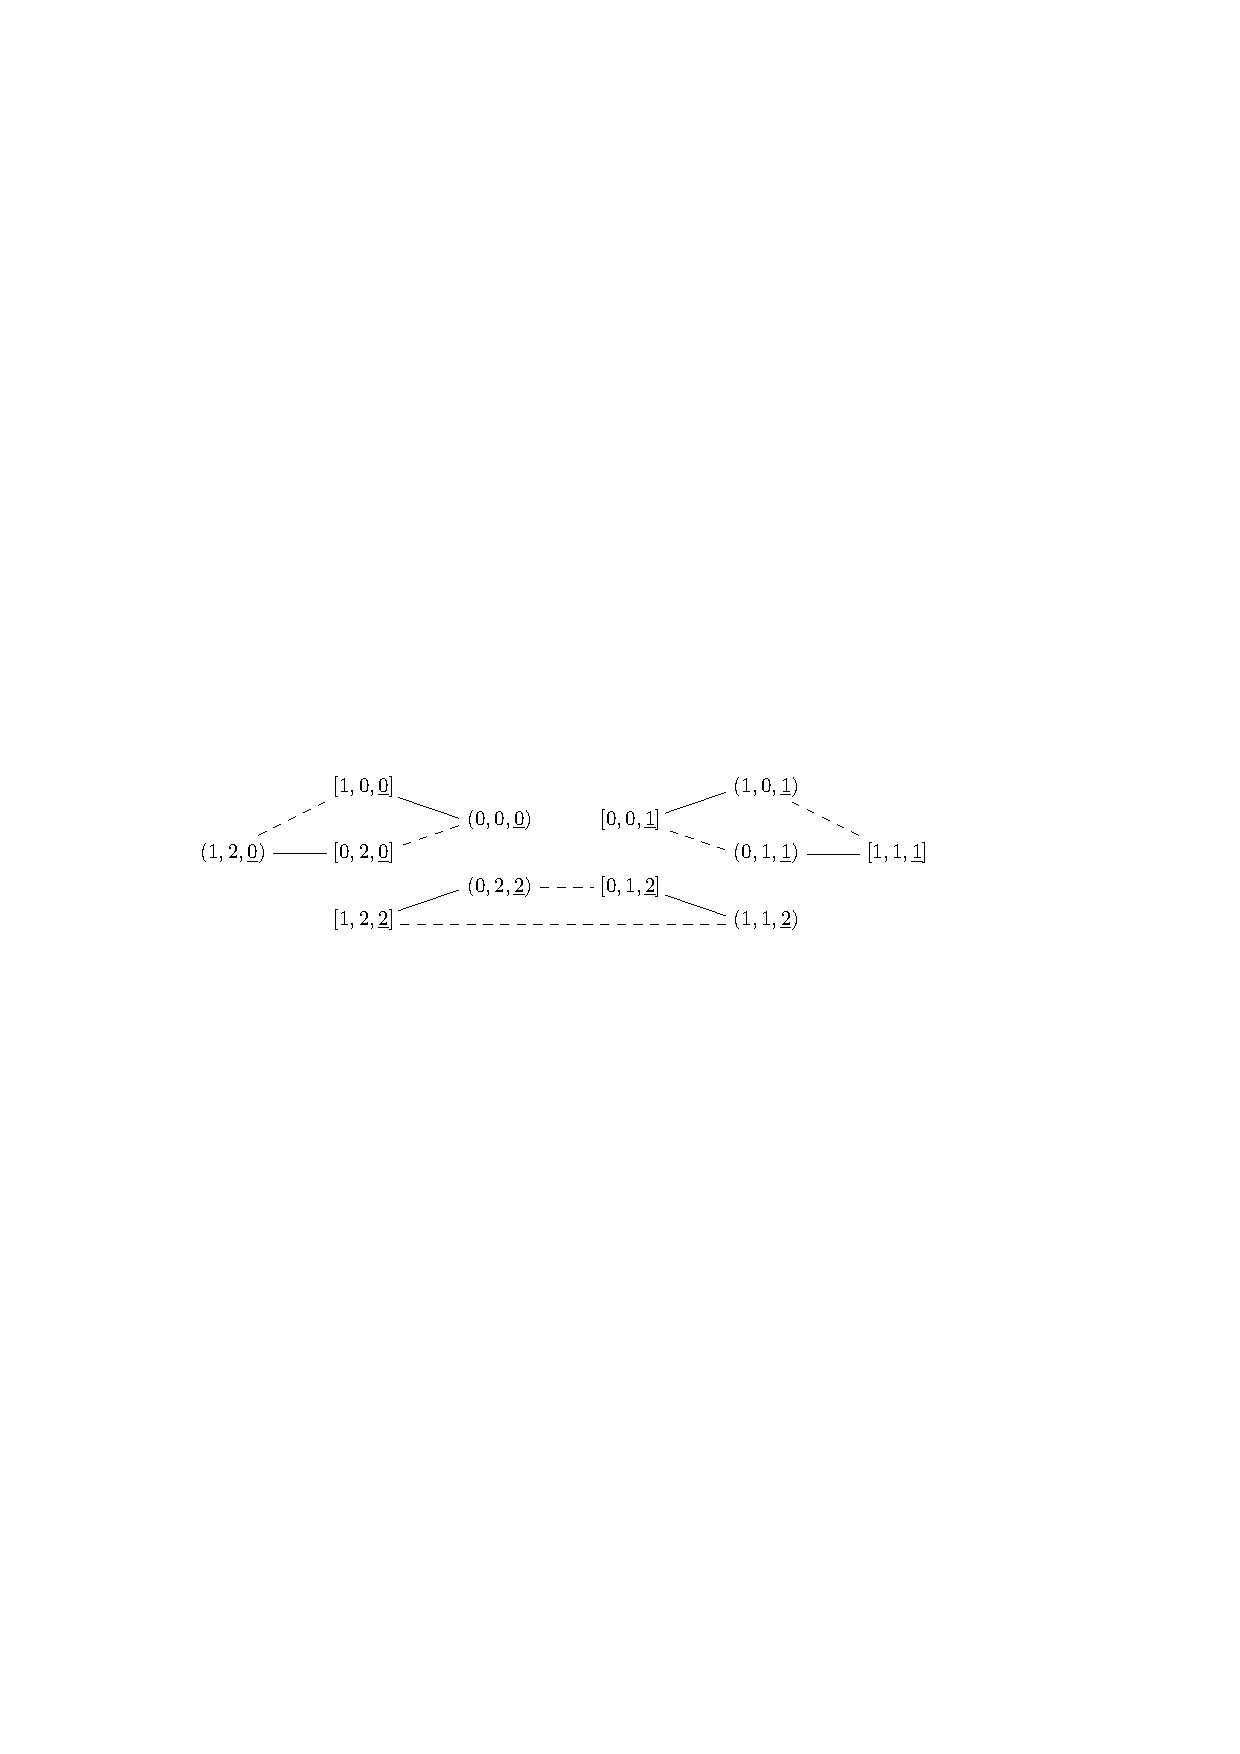
\includegraphics[width=0.9\textwidth]{img/separated.pdf}
\caption{2-color cycles in a separated latin bitrade.}
\label{fig:separated-graph}
\end{figure}
\end{exmp}%

%\begin{lem}
%\label{lem:3-coloring}
%Let $G$ be a planar cubic bipartite graph. Then there exists unique face 3-coloring of $G$.
%\end{lem}
%\begin{proof}
%This result was already known to Heawood. A proof of it can be found in \cite{Tutte48}.
%\end{proof}

The following results regarding the relation of a latin bitrade and its graph in the planar case are due to Cavenagh and Lisoněk \cite{CavenaghLisonek08}. We state them without a proof. They considered unordered latin squares $\{T,T'\}$. 

\begin{defn}
A graph is \emph{Eulerian} if each vertex is of even degree. \emph{A triangulation} of a plane is an embedding of a graph into the plane such that every face is a triangle.
\end{defn}

\begin{lem}
Dual of the graph of a connected spherical latin bitrade is an Eulerian triangulation.
\end{lem}
\begin{proof}
Trivial.
\end{proof}

\begin{thm}
\label{thm:connected-spherical-separated}
There is a bijection between the main classes of connected separated spherical unordered latin bitrades of size $v-2$ and the isomorphism classes of planar Eulerian triangulations on $v$ vertices.
\end{thm}%

\begin{cor}
\label{cor:connected-spherical-separated}
There is an algorithm to reconstruct a connected separated spherical latin bitrade $(T,T')$ from its graph up to isotopy, conjugacy, and switch of the roles of $T$ and $T'$.
\end{cor}%



